
\sectioncounter{5}
  \section{函数的图象}

  \subsection{知识梳理}
  \myindex{函数的图象} (graph of functions) 用图形来表示函数的自变量和因变量之间的关系, 即表示其对应法则.
  函数图象最基本的画法是\myemph{描点法}.
  对常见的函数, 如一次函数, 二次函数, 反比例函数, 幂函数, 指数函数, 对数函数, 三角函数, 需掌握它们图象的画法. 与函数的图象密切相关的函数性质有单调性和奇偶性.
  
  函数图象的第二种画法是利用\myindex{图象变换} (graph tranformation), 如要得到 $y=(x-1)^2$ 的图象, 
  只需把 $y=x^2$ 的图象向右平移 1 个单位长度. 设函数为 $y=f(x)$, $a>0$,
  常用的图象变换法则如下 (考虑变换前后对应点的坐标可知):
  
  向左平移 $a$ 个单位长度: $f(x)\rightarrow f(x+a)$;
  
  向右平移 $a$ 个单位长度: $f(x)\rightarrow f(x-a)$;
  
  向上平移 $a$ 个单位长度: $f(x)\rightarrow f(x)+a$;
  
  向下平移 $a$ 个单位长度: $f(x)\rightarrow f(x)-a$;
  
  关于 $y$~轴对称: $f(x)\rightarrow f(-x)$;
  \mymarginpar{关于 $x=a$ 轴对称: $f(x)\rightarrow f(2a-x)$;\\
    关于 $y=b$ 轴对称: $f(x)\rightarrow 2b-f(x)$.}
    
  关于 $y$~轴对称: $f(x)\rightarrow f(-x)$;
  
  关于 $x$~轴对称: $f(x)\rightarrow -f(x)$;
  
  纵坐标不变, 横坐标变为原来的 $a$ 倍: $f(x)\rightarrow f\Big(\frac{x}a\Big)$;
  
  横坐标不变, 纵坐标变为原来的 $a$ 倍: $f(x)\rightarrow af(x)$.\\
  前两个法则也简记为 ``左加右减'', 倒数第二个法则描述的是图象相对 $y$~轴的拉伸或压缩,
  最后一个法则描述的是图象相对 $x$~轴的拉伸或压缩. 
  注意, 以上法则均是对 $x$ 或 $f(x)$ (即 $y$) 的整体变换, 
  例如 $f(2x)$ 往左平移 1~个单位长度, 得到 $f(2(x+1))$ 即 $f(2x+2)$.
  
  思考: $|f(x)|$ 与 $f(x)$, $f(|x|)$ 与 $f(x)$ 的图象关系分别是什么?
  \mymarginpar{把 $f(x)$ 图象中 $x$~轴下方的部分关于 $x$~轴作对称图形 (翻折), $x$~轴上方的部分不变, 可得到  $|f(x)|$ 的图象;\\[4pt]
    把 $f(x)$ 图象中 $y$~轴左侧的部分删去, $y$~轴左侧的部分不变并关于 $y$~轴作对称图形 (翻折), 可得到  $f(|x|)$ 的图象.}
  
  函数图象的第三种画法是利用导数确定单调性和极值点, 再描点作图.
  
  \lianxi
  \begin{exercise}
    函数 $y=|x+1|$ 的图象是\,?
  \end{exercise}

  \beginsolution
     利用 $y=|x|$ 或 $y=x+1$ 的图象变换可得, 也可先写为分段函数再作图.
    \begin{center}
    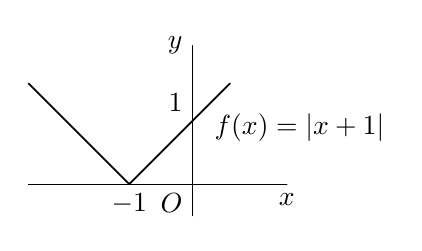
\begin{tikzpicture}[line cap=round,line join=round,scale=0.8]
      \draw[\myaxisarrow] (-2.6,0) -- (1.5,0) node[below] {$x$};
      \draw[\myaxisarrow] (0,-0.5) -- (0,2.2) node[left] {$y$};
      \draw[line width=0.6pt,smooth,samples=100] plot[domain=-2.6:0.6](\x,{abs(\x+1)});
      \draw (-1,0) node[below] {$-1$}
        (0,0) node[anchor=north east] {$O$}
        (0,1) node[anchor=south east] {$1$}
        (0.2,0.9) node[right] {$f(x)=|x+1|$};
    \end{tikzpicture}
    \end{center}
  \endsolution
  
  \begin{exercise}
    图~\ref{fig-190414-2045}~中, 不能表示函数关系的是\,?(填序号)
    \begin{figure}[htb]
    \small
    \centering
    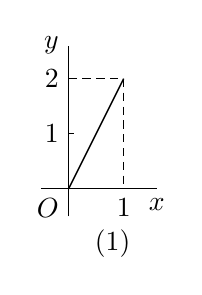
\begin{tikzpicture}[scale=0.7]
      \draw[\myaxisarrow] (-0.5,0) -- (1.6,0) node[below] {$x$};
      \draw[\myaxisarrow] (0,-0.5) -- (0,2.6) node[left] {$y$};
      \draw[line width=0.5pt,densely dashed] 
        (0,2)--(1,2)--(1,0);
      \draw[line width=0.5pt] (0,0)--(1,2);
      
      \draw (1,0) node[below] {$1$};
      \draw (0,2) node[left] {$2$};
      \draw[line width=0.5pt] (0,1)--(0.1,1);
      \draw (0,1) node[left] {$1$};
      \draw (0,0) node[anchor=north east] {$O$};
      \draw (0.8,-1) node {(1)};
    \end{tikzpicture}\hskip0.4cm
    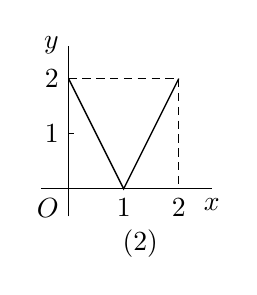
\begin{tikzpicture}[scale=0.7]
      \draw[\myaxisarrow] (-0.5,0) -- (2.6,0) node[below] {$x$};
      \draw[\myaxisarrow] (0,-0.5) -- (0,2.6) node[left] {$y$};
      \draw[line width=0.5pt,densely dashed] 
        (0,2)--(2,2)--(2,0);
      \draw[line width=0.5pt] (0,2)--(1,0)--(2,2);
      
      \draw (1,0) node[below] {$1$};
      \draw (2,0) node[below] {$2$};
      \draw (0,2) node[left] {$2$};
      \draw[line width=0.5pt] (0,1)--(0.1,1);
      \draw (0,1) node[left] {$1$};
      \draw (0,0) node[anchor=north east] {$O$};
      \draw (1.3,-1) node {(2)};
    \end{tikzpicture}\hskip0.4cm
    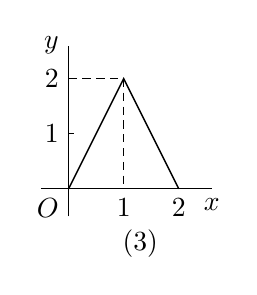
\begin{tikzpicture}[scale=0.7]
      \draw[\myaxisarrow] (-0.5,0) -- (2.6,0) node[below] {$x$};
      \draw[\myaxisarrow] (0,-0.5) -- (0,2.6) node[left] {$y$};
      \draw[line width=0.5pt,densely dashed] 
        (0,2)--(1,2)--(1,0);
      \draw[line width=0.5pt] (0,0)--(1,2)--(2,0);
      
      \draw (1,0) node[below] {$1$};
      \draw (2,0) node[below] {$2$};
      \draw (0,2) node[left] {$2$};
      \draw[line width=0.5pt] (0,1)--(0.1,1);
      \draw (0,1) node[left] {$1$};
      \draw (0,0) node[anchor=north east] {$O$};
      \draw (1.3,-1) node {(3)};
    \end{tikzpicture}\hskip0.4cm
    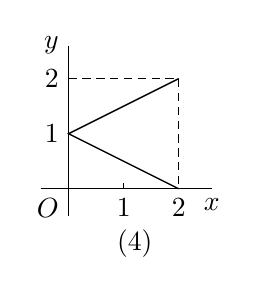
\begin{tikzpicture}[scale=0.7]
      \draw[\myaxisarrow] (-0.5,0) -- (2.6,0) node[below] {$x$};
      \draw[\myaxisarrow] (0,-0.5) -- (0,2.6) node[left] {$y$};
      \draw[line width=0.5pt,densely dashed] 
        (0,2)--(2,2)--(2,0);
      \draw[line width=0.5pt] (2,0)--(0,1)--(2,2);
      
      \draw[line width=0.5pt] (1,0)--(1,0.1);
      \draw (1,0) node[below] {$1$};
      \draw (2,0) node[below] {$2$};
      \draw (0,2) node[left] {$2$};
      \draw (0,1) node[left] {$1$};
      \draw (0,0) node[anchor=north east] {$O$};
      \draw (1.2,-1) node {(4)};
    \end{tikzpicture}
    \caption{}\label{fig-190414-2045}
    \end{figure}
  \end{exercise}

  \beginsolution
    $x$ 与 $y$ 不可一对二, 故 (4) 不能表示函数关系.
  \endsolution
  
  \begin{exercise}
    函数 $y=x^2+2x+1$ 的图象可以由 $y=x^2$ 的图象如何平移得到\,?
  \end{exercise}

  \beginsolution
    $y=(x+1)^2$, 其图象可由 $y=x^2$ 的图象向左平移 $1$~个单位长度得到.
    
    \varexercise 函数 $y=x^2+2x$ 的图象可以由 $y=x^2$ 的图象如何平移得到\,?
    
    $y=(x+1)^2-1$, 其图象可由 $y=x^2$ 的图象向左平移 $1$~个单位长度, 再向下平移 $1$~个单位长度得到.
    
    \varexercise 函数 $y=x^2-2x$ 的图象可以由 $y=x^2$ 的图象如何平移得到\,?
    
    $y=(x-1)^2-1$, 其图象可由 $y=x^2$ 的图象向右平移 $1$~个单位长度, 再向下平移 $1$~个单位长度得到.
  \endsolution
  
  \begin{exercise}
    已知函数 $f(x)$ 是定义在 $(-3,3)$ 上的偶函数, 
    当 $0\leqslant x<3$ 时, 
    $f(x)$ 的图象如图~\ref{fig-190414-2055} 所示, 
    那么不等式 $x\cdot f(x)<0$ 的解集是\,?
    \begin{figure}[htb]
    \small
    \centering
    \begin{tikzpicture}[scale=0.7]
      \draw[\myaxisarrow] (-3.5,0) -- (3.7,0) node[below] {$x$};
      \draw[\myaxisarrow] (0,-1.5) -- (0,1.7) node[left] {$y$};
      \draw[line width=0.6pt,smooth,samples=100,domain=0:3] 
        plot(\x,{-cos(\x*90)});
      \draw[line width=0.5pt] (1,0) node[below,xshift=2pt] {$1$} --(1,0.15)
        (2,0) node[below] {$2$} --(2,0.15);
      \draw[fill=white] (3,0) circle(2pt) node[below] {$3$};
      \draw (0,0) node[anchor=north east] {$O$};
    \end{tikzpicture}
    \caption{}\label{fig-190414-2055}
    \end{figure}
  \end{exercise}

  \beginsolution
    补全 $f(x)$ 的图象, 见右图. $x\cdot f(x)<0$ 表明 $x$ 和 $f(x)$ 异号, 所以 $x\in (-3,-1)\cup (0,1)$.
    \mymarginpar{\centering
      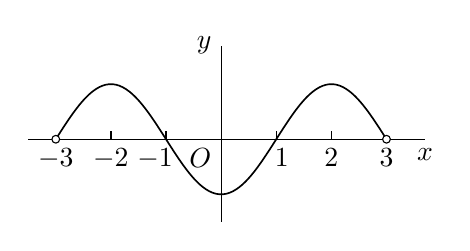
\begin{tikzpicture}[scale=0.7]
      \draw[\myaxisarrow] (-3.5,0) -- (3.7,0) node[below] {$x$};
      \draw[\myaxisarrow] (0,-1.5) -- (0,1.7) node[left] {$y$};
      \draw[line width=0.6pt,smooth,samples=100,domain=-3:3] 
        plot(\x,{-cos(\x*90)});
      \foreach \i in {-2,-1,1,2}
      {\draw[line width=0.5pt] (\i,0)--(\i,0.15);}
      \draw[fill=white] (-3,0) circle(2pt) node[below] {$-3$}
        (3,0) circle(2pt) node[below] {$3$};
      \draw (-2,0) node[below] {$-2$} (2,0) node[below] {$2$} 
        (-1,0) node[below,xshift=-4pt] {$-1$} 
        (1,0) node[below,xshift=2pt] {$1$} 
        (0,0) node[anchor=north east] {$O$};
      \end{tikzpicture}}
  \endsolution
  
  \subsection{要点导学\quad 各个击破}
  \subsubsection{画函数的图象}
  \begin{example}
    根据所给定义域, 画出函数 $y=x^2-2x+2$ 的图象.
    
    (1) $x\in \mathbb{R}$; \qquad
    (2) $x\in (-1,2]$;\qquad 
    (3) $x\in (-1,2]$ 且 $x\in\mathbb{Z}$.
  \end{example}

  \beginsolution
    $y=(x-1)^2+1$, 各小题图象如下:
    \begin{center}
    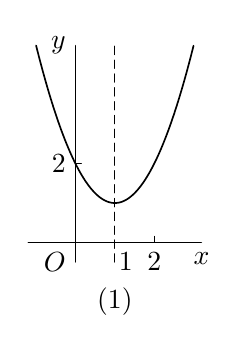
\begin{tikzpicture}[line cap=round,line join=round,scale=0.5]
      \draw[\myaxisarrow] (-1.2,0) -- (3.2,0) node[below] {$x$};
      \draw[\myaxisarrow] (0,-0.5) -- (0,5) node[left] {$y$};
      \draw[line width=0.6pt,smooth,samples=100,domain=-1:3] 
        plot(\x,{(\x-1)^2+1});
      \draw[densely dashed] (1,-0.5)--(1,5);
      \draw (0,0) node[anchor=north east] {$O$} 
        (1,0) node[below,xshift=4pt] {$1$}
        (2,0) node[below] {$2$}--(2,0.15)
        (0,2) node[left] {$2$}--(0.15,2)
        (1,-1.5) node {(1)};
    \end{tikzpicture}\qquad
    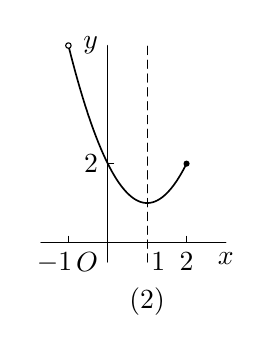
\begin{tikzpicture}[line cap=round,line join=round,scale=0.5]
      \draw[\myaxisarrow] (-1.7,0) -- (3,0) node[below] {$x$};
      \draw[\myaxisarrow] (0,-0.5) -- (0,5) node[left] {$y$};
      \draw[line width=0.6pt,smooth,samples=100,domain=-1:2] 
        plot(\x,{(\x-1)^2+1});
      \draw[densely dashed] (1,-0.5)--(1,5);
      \draw (0,0) node[anchor=north east] {$O$} 
        (-1,0) node[below,xshift=-5pt] {$-1$}--(-1,0.15)
        (1,0) node[below,xshift=4pt] {$1$} 
        (2,0) node[below] {$2$}--(2,0.15)
        (0,2) node[left] {$2$}--(0.15,2)
        (1,-1.5) node {(2)};
      \draw[fill=black] (2,2) circle(1.8pt);
      \draw[fill=white] (-1,5) circle(2pt);
    \end{tikzpicture}\qquad
    \begin{tikzpicture}[line cap=round,line join=round,scale=0.5]
      \draw[\myaxisarrow] (-1,0) -- (3,0) node[below] {$x$};
      \draw[\myaxisarrow] (0,-0.5) -- (0,5) node[left] {$y$};
      \draw[fill=black] (0,0) node[anchor=north east] {$O$} 
        (1,0) node[below] {$1$}--(1,0.15)
        (2,0) node[below] {$2$}--(2,0.15)
        (0,2) circle(1.7pt) node[left] {$2$}--(0.15,2)
        (1,1) circle(1.7pt) (2,2) circle(1.8pt) 
        (1,-1.5) node {(3)};
    \end{tikzpicture}
    \end{center}
  \endsolution
  
  \lianxi
  \begin{exercise}[s]
    作函数 $y=\dfrac{3x+4}{x+2}$ 的图象.
  \end{exercise}

  \beginsolution
    $y=3-\frac2{x+2}$, 图象可由 $y=-\frac2x$ 的图象平移得到.
    \mymarginpar{作图时先画渐近线.}
    \begin{center}
    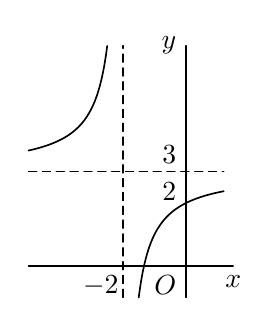
\begin{tikzpicture}[line cap=round,line join=round,scale=0.4]
      \draw[\myaxisarrow] (-5,0) -- (1.5,0) node[below] {$x$};
      \draw[\myaxisarrow] (0,-1) -- (0,7) node[left] {$y$};
      \draw[line width=0.6pt,smooth,samples=100] 
        plot[domain=-5:-2.5](\x,{(3*\x+4)/(\x+2)})
        plot[domain=-1.5:1.2](\x,{(3*\x+4)/(\x+2)});
      \draw[densely dashed] (-2,-1)--(-2,7) (-5,3)--(1.2,3);
      \draw (0,0) node[anchor=north east] {$O$} 
        (-2,0) node[below,xshift=-8pt] {$-2$}
        (0,3) node[left,yshift=6pt] {$3$}
        (0,2) node[left,yshift=4pt] {$2$};
    \end{tikzpicture}
    \end{center}
  \endsolution
  
  \subsubsection{函数图象的变换}
  \begin{example}
    说明指数函数 $y=3^x$ 的图象怎样变换可得到以下函数的图象:
    
    (1) $y=3^{x+1}+2$;\qquad  (2) $y=3^{-x}+2$;\qquad
    (3) $y=3^{-x-1}+2$.
  \end{example}

  \beginsolution
    (1) 向左平移 $1$ 个单位长度, 再向上平移 $2$ 个单位长度;
    \mymarginpar{作图时先画渐近线, 三个图中的渐近线均为 $y=2$.}
    (2) 关于 $y$~轴作对称图形, 再向上平移 $2$ 个单位长度;
    (3) 关于 $x$~轴作对称图形, 向左平移 $1$ 个单位长度, 再向上平移 $2$ 个单位长度.
  \endsolution
  
  \lianxi
  \begin{exercise}[s]
    已知函数 $y=f(x+1)$ 的图象过点 $(3,2)$, 那么函数 $f(x)$ 的
    图象一定过哪个点\,?其关于 $x$ 轴的对称图形一定过哪个点\,?
  \end{exercise}

  \beginsolution
    $2=f(3+1)=f(4)$, 故 $f(x)$ 的图象一定过点 $(4,2)$, 其关于 $x$ 轴的对称图形一定过点 $(-4,2)$.
    
    \varexercise $f(x)$ 同上, 则 $y=f(2x)$ 的图象一定过哪个点?
    
    由 $2=f(4)=f(2\cdot 2)$ 知, $y=f(2x)$ 的图象一定过点 $(2,2)$.
  \endsolution
  
  \subsubsection{函数图象的应用}
  \begin{example}
    已知关于 $x$ 的方程 $|x^2 -4x+3|=mx$ 有四个不等实根, 求实数 $m$ 的取值范围.
  \end{example}

  \beginsolution
    方法一: 先作出 $f(x)=|x^2-4x+3|$ 和 $g(x)=mx$ 的图象. 
    因为 $g(x)$ 的图象为过原点的直线, 由图象知, 当 $g(x)$ 与 $f(x)$ 在 $[1,3]$ 上的图象相切时, $f(x)=g(x)$ 恰有三个根. 此时 $-(x^2-4x+3)=mx$ 即 $x^2+(m-4)x+3=0$恰在 $[1,3]$ 上有两个相等实根, 且 $m>0$, 则
    \mymarginpar{\centering
      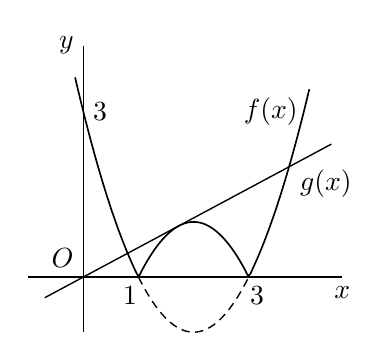
\begin{tikzpicture}[scale=0.7]
      \draw[\myaxisarrow] (-1,0) -- (4.7,0) node[below] {$x$};
      \draw[\myaxisarrow] (0,-1) -- (0,4.2) node[left] {$y$};
      \draw[line width=0.6pt,smooth,samples=100,domain=-0.15:4.1] 
        plot(\x,{abs((\x)^2-4*\x+3)});
      \draw[line width=0.5pt,smooth,samples=100,domain=1:3,densely dashed] 
        plot(\x,{(\x)^2-4*\x+3});
      \draw[line width=0.5pt,smooth,samples=100,domain=-0.7:4.5] 
        plot(\x,{(4-2*sqrt(3))*\x});
      \draw (1,0) node[below,xshift=-3pt] {$1$} 
        (3,0) node[below,xshift=3pt] {$3$}
        (0,3) node[right] {$3$} (0,0) node[anchor=south east] {$O$}
        (3.4,3) node {$f(x)$} (4.4,1.7) node {$g(x)$};
      \end{tikzpicture}}
    \[(m-4)^2-4\cdot 3=0, \text{\ 且\ } -\frac{m-4}2\in[1,3],\]
    解得 $m=4-2\sqrt3$. 再由图象知, $f(x)=g(x)$ 有四个不等实根时, $m\in(0,4-2\sqrt3)$.
    
    方法二: 若 $m\leqslant 0$, 则 $x\leqslant 0$, 方程为 $x^2-4x+3=mx$, 
    \mymarginpar{形如 $y=x+\frac{k}x$ ($k>0$) 的函数有时也被称为 ``对勾函数'', 图象有两条渐近线, 为双曲线.}
    至多有两个不等实根, 与题意不符. 所以 $m>0$ 且 $x>0$, 方程改写为
    \[m=\Big|x+\frac3x-4\Big|,\quad x>0.\]
    作 $h(x)=\Big|x+\frac3x-4\Big|$ 的图象 (可由 $y=x+\frac3x$ 的图象经变换得到).
    \mymarginpar{由两种方法都可以得到, 若原方程恰有三个实根, 则 $m=4-2\sqrt3$.}
    \begin{center}
    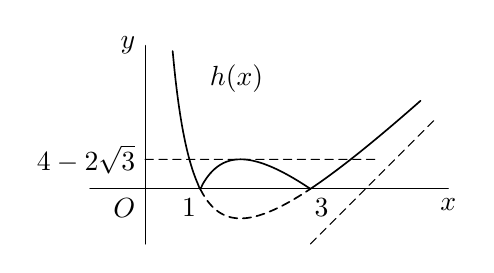
\begin{tikzpicture}[line cap=round,line join=round,scale=0.7]
      \draw[\myaxisarrow] (-1,0) -- (5.5,0) node[below] {$x$};
      \draw[\myaxisarrow] (0,-1) -- (0,2.6) node[left] {$y$};
      \draw[line width=0.6pt,smooth,samples=100] 
        plot[domain=0.5:5](\x,{abs(\x+3/(\x)-4)});
      \draw[line width=0.6pt,smooth,samples=100,densely dashed]
        plot[domain=1:3](\x,{\x+3/(\x)-4});
      \draw[densely dashed] (3,-1)--(5.3,1.3) 
        (0,{4-2*sqrt(3)})--(4.2,{4-2*sqrt(3)});
      \draw (0,0) node[anchor=north east] {$O$} 
        (1,0) node[below,xshift=-4pt] {$1$}
        (3,0) node[below,xshift=4pt] {$3$}
        (0,{4-2*sqrt(3)}) node[left] {$4-2\sqrt3$}
        (1,2) node[right] {$h(x)$};
    \end{tikzpicture}
    \end{center}
    故 $h(x)=m$ 有四个不等实根时, $m\in(0,4-2\sqrt3)$.
  \endsolution
  
  \lianxi
  \begin{exercise}[s]
    对于每一个实数 $x$, $f(x)$ 取 $4-x$, $x+2$, $3^x$ 三个值中最小的值,
    则 $f(x)$ 的最大值为\,?
  \end{exercise}

  \beginsolution
    作函数 $y=4-x$, $y=x+2$, $y=3^x$ 的图象, 对比可知 $f_{\max}= f(1)=3$.
    \mymarginpar{\centering
    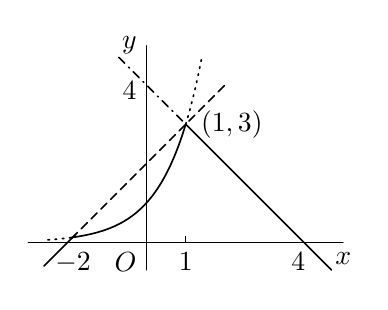
\begin{tikzpicture}[line cap=round,line join=round,scale=0.5]
      \draw[\myaxisarrow] (-3,0) -- (5,0) node[below] {$x$};
      \draw[\myaxisarrow] (0,-0.7) -- (0,5) node[left] {$y$};
      \draw[line width=0.6pt,smooth,samples=100] 
        plot[domain=-1.9:1](\x,{3^(\x)});
      \draw[line width=0.6pt,smooth,samples=100,dotted]
        plot[domain=-2.5:-1.9](\x,{3^(\x)})
        plot[domain=1:1.4](\x,{3^(\x)});
      \draw[line width= 0.6pt] (-2.6,-0.6)--(-1.8,0.2) (1,3)--(4.7,-0.7);
      \draw[densely dashed,line width=0.6pt] (-1.9,0.1)--(2,4);
      \draw[dash dot,line width=0.6pt] (-0.7,4.7)--(1,3);
      \draw (0,0) node[anchor=north east] {$O$} 
        (-2,0) node[below,xshift=2pt] {$-2$}
        (4,0) node[below,xshift=-2pt] {$4$}
        (1,0) node[below] {$1$} --(1,0.15)
        (0,4) node[left,yshift=-2pt] {$4$}
        (1,3) node[right,xshift=2pt] {$(1,3)$};
    \end{tikzpicture}}
  \endsolution
  
  \subsubsection{课堂评价}
  \begin{exercise}
    怎样由函数 $y= \lg\dfrac{x+3}{10}$ 的图象得到 $y= \lg x$ 的图象\,?
  \end{exercise}

  \beginsolution
    $y=\lg(x+3)-1$, 向左平移 $3$~个单位长度, 再向下平移 $1$~个单位长度.
  \endsolution
  
  \begin{exercise}
    函数 $f(x)= \ln x$ 与 $g(x)=x^2 -4x+4$ 的图象的交点个数为\,?
  \end{exercise}

  \beginsolution
    作草图可知, 共有两个交点.
    \mymarginpar{进一步分析可知, 两个交点横坐标分别在 $[1,2]$ 和 $[3,4]$ 内.}
  \endsolution

  \begin{exercise}
    已知函数 $f(x)= x|x-2|$, 解不等式 $f(x)\leqslant 1$.
  \end{exercise}

  \beginsolution
    分类讨论知
    \[f(x)=\begin{cases}
      x(2-x),& x\leqslant 2,\\
      x(x-2),& x>2,
      \end{cases}\]
    再作 $f(x)$ 图象. 因为 $f(x)\leqslant 1=f(1+\sqrt2)$, 由图象知, $x\in(-\infty,1+\sqrt2]$.
    \mymarginpar{\centering
    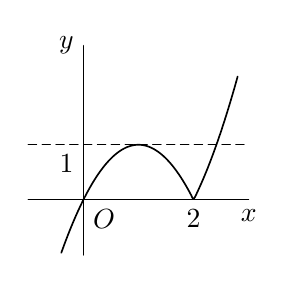
\begin{tikzpicture}[line cap=round,line join=round,scale=0.7]
      \draw[\myaxisarrow] (-1,0) -- (3,0) node[below] {$x$};
      \draw[\myaxisarrow] (0,-1) -- (0,2.8) node[left] {$y$};
      \draw[line width=0.6pt,smooth,samples=100] 
        plot[domain=-0.4:2.8](\x,{\x*abs(\x-2)});
      \draw[densely dashed] (-1,1)--(3,1);
      \draw (0,0) node[anchor=north west] {$O$} 
        (2,0) node[below] {$2$} (0,1) node[anchor=north east] {$1$};
    \end{tikzpicture}}
  \endsolution
  
  \subsection{课后练习}
  \begin{exercise}
    怎样由函数 $y=\log_2 x$ 的图象得到 $y=\log_2 \sqrt{x-1}$ 的图象\,?
  \end{exercise}

  \beginsolution
    后一函数可化为 $y=\frac12\log_2 (x-1)$, 所以可由 $y=\log_2 x$ 的图象向右平移 $1$~个单位长度, 然后横坐标不变, 纵坐标变为原来的 $\frac12$ 而得到.
  \endsolution
  
  \begin{exercise}
    若函数 $f(x)$ 的图象向右平移 $1$ 个单位长度所得图象与 
    $y=\mathrm{e}^x$ 的图象关于 $y$ 轴对称, 则 $f(x)=$\,?
  \end{exercise}

  \beginsolution
    $y=\mathrm{e}^x$ 的图象关于 $y$~轴对称, 再向左平移 $1$~个单位长度, 可得 $f(x)=\mathrm{e}^{-(x+1)}$.
  \endsolution
  
  \begin{exercise}
    如图~\ref{fig-190414-2110}, 在同一平面直角坐标系中, 
    函数 $f(x)=x^a$ ($x>0$), $g(x)=\log_a x$ 的图象可能是$\underline{\qquad}$.(填序号)
    \begin{figure}[htb]
    \small
    \centering
    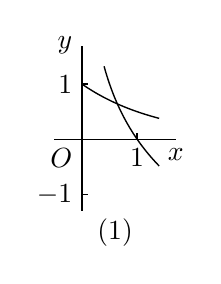
\begin{tikzpicture}[scale=0.7]
      \draw[\myaxisarrow] (-0.5,0) -- (1.7,0) node[below] {$x$};
      \draw[\myaxisarrow] (0,-1.3) -- (0,1.7) node[left] {$y$};
      \draw[line width=0.5pt,smooth,samples=100,domain=0:1.4] 
        plot(\x,{0.5^(\x)});
      \draw[line width=0.5pt,smooth,samples=100,domain=0.4:1.4] 
        plot(\x,{-ln(\x)/ln(2)});
      
      \draw[line width=0.5pt] (1,0)--(1,0.11);
      \draw (1,0) node[below] {$1$};
      \draw[line width=0.5pt] (0,1)--(0.11,1);
      \draw (0,1) node[left] {$1$};
      \draw[line width=0.5pt] (0,-1)--(0.11,-1);
      \draw (0,-1) node[left] {$-1$};
      \draw (0,0) node[anchor=north east] {$O$};
      \draw (0.6,-1.7) node {(1)};
    \end{tikzpicture}\hskip0.6cm
    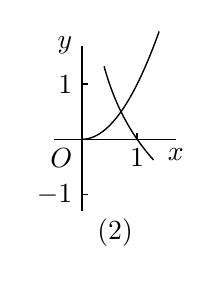
\begin{tikzpicture}[scale=0.7]
      \draw[\myaxisarrow] (-0.5,0) -- (1.7,0) node[below] {$x$};
      \draw[\myaxisarrow] (0,-1.3) -- (0,1.7) node[left] {$y$};
      \draw[line width=0.5pt,smooth,samples=100,domain=0:1.4] 
        plot(\x,{(\x)^2});
      \draw[line width=0.5pt,smooth,samples=100,domain=0.4:1.3] 
        plot(\x,{-ln(\x)/ln(2)});
      
      \draw[line width=0.5pt] (1,0)--(1,0.11);
      \draw (1,0) node[below] {$1$};
      \draw[line width=0.5pt] (0,1)--(0.11,1);
      \draw (0,1) node[left] {$1$};
      \draw[line width=0.5pt] (0,-1)--(0.11,-1);
      \draw (0,-1) node[left] {$-1$};
      \draw (0,0) node[anchor=north east] {$O$};
      \draw (0.6,-1.7) node {(2)};
    \end{tikzpicture}\hskip0.6cm
    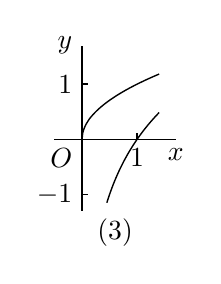
\begin{tikzpicture}[scale=0.7]
      \draw[\myaxisarrow] (-0.5,0) -- (1.7,0) node[below] {$x$};
      \draw[\myaxisarrow] (0,-1.3) -- (0,1.7) node[left] {$y$};
      \draw[line width=0.5pt,smooth,samples=100,domain=0:1.4] 
        plot(\x,{(\x)^0.5});
      \draw[line width=0.5pt,smooth,samples=100,domain=0.45:1.4] 
        plot(\x,{ln(\x)/ln(2)});
      
      \draw[line width=0.5pt] (1,0)--(1,0.11);
      \draw (1,0) node[below] {$1$};
      \draw[line width=0.5pt] (0,1)--(0.11,1);
      \draw (0,1) node[left] {$1$};
      \draw[line width=0.5pt] (0,-1)--(0.11,-1);
      \draw (0,-1) node[left] {$-1$};
      \draw (0,0) node[anchor=north east] {$O$};
      \draw (0.6,-1.7) node {(3)};
    \end{tikzpicture}\hskip0.6cm
    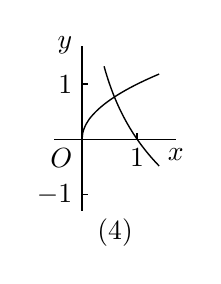
\begin{tikzpicture}[scale=0.7]
      \draw[\myaxisarrow] (-0.5,0) -- (1.7,0) node[below] {$x$};
      \draw[\myaxisarrow] (0,-1.3) -- (0,1.7) node[left] {$y$};
      \draw[line width=0.5pt,smooth,samples=100,domain=0:1.4] 
        plot(\x,{(\x)^0.5});
      \draw[line width=0.5pt,smooth,samples=100,domain=0.4:1.4] 
        plot(\x,{-ln(\x)/ln(2)});
      \draw[line width=0.5pt] (1,0)--(1,0.11);
      \draw (1,0) node[below] {$1$};
      \draw[line width=0.5pt] (0,1)--(0.11,1);
      \draw (0,1) node[left] {$1$};
      \draw[line width=0.5pt] (0,-1)--(0.11,-1);
      \draw (0,-1) node[left] {$-1$};
      \draw (0,0) node[anchor=north east] {$O$};
      \draw (0.6,-1.7) node {(4)};
    \end{tikzpicture}
    \caption{}\label{fig-190414-2110}
    \end{figure}
  \end{exercise}

  \beginsolution
    分 $0<a<1$ 和 $a>1$ 两种情况作图, 可知选 (4).
    \mymarginpar{\centering
    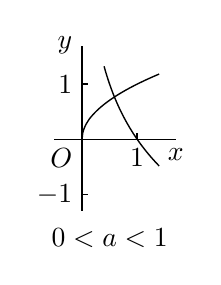
\begin{tikzpicture}[scale=0.7]
      \draw[\myaxisarrow] (-0.5,0) -- (1.7,0) node[below] {$x$};
      \draw[\myaxisarrow] (0,-1.3) -- (0,1.7) node[left] {$y$};
      \draw[line width=0.5pt,smooth,samples=100,domain=0:1.4] 
        plot(\x,{(\x)^0.5});
      \draw[line width=0.5pt,smooth,samples=100,domain=0.4:1.4] 
        plot(\x,{-ln(\x)/ln(2)});
      \draw[line width=0.5pt] (1,0)--(1,0.11) 
        (0,1)--(0.11,1) (0,-1)--(0.11,-1);
      \draw (1,0) node[below] {$1$} 
        (0,1) node[left] {$1$}
        (0,-1) node[left] {$-1$} 
        (0,0) node[anchor=north east] {$O$}
        (0.5,-1.8) node {$0<a<1$};
    \end{tikzpicture}\qquad
    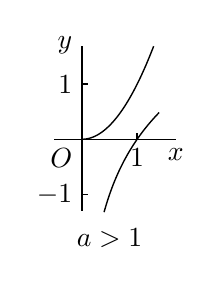
\begin{tikzpicture}[scale=0.7]
      \draw[\myaxisarrow] (-0.5,0) -- (1.7,0) node[below] {$x$};
      \draw[\myaxisarrow] (0,-1.3) -- (0,1.7) node[left] {$y$};
      \draw[line width=0.5pt,smooth,samples=100,domain=0:1.3] 
        plot(\x,{(\x)^2});
      \draw[line width=0.5pt,smooth,samples=100,domain=0.4:1.4] 
        plot(\x,{ln(\x)/ln(2)});
      \draw[line width=0.5pt] (1,0)--(1,0.11) 
        (0,1)--(0.11,1) (0,-1)--(0.11,-1);
      \draw (1,0) node[below] {$1$} 
        (0,1) node[left] {$1$}
        (0,-1) node[left] {$-1$} 
        (0,0) node[anchor=north east] {$O$}
        (0.5,-1.8) node {$a>1$};
    \end{tikzpicture}}
  \endsolution
  
  \begin{exercise}
    已知定义域为 $(-\infty ,0)\cup (0,+\infty)$ 的函数 $f(x)$ 是偶函数,
    且在 $(-\infty ,0)$ 上是单调增函数. 若 $f(-3)=0$, 
    则不等式 $\frac{x}{f(x)}<0$ 的解集是\,?
  \end{exercise}

  \beginsolution
    作 $f(x)$ 图象的大致示意图. 
    \mymarginpar{\centering
    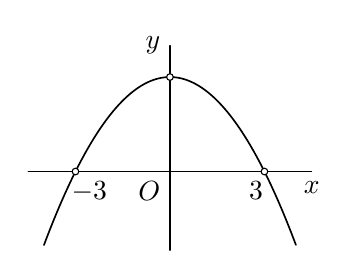
\begin{tikzpicture}[line cap=round,line join=round,scale=0.4]
      \draw[\myaxisarrow] (-4.5,0) -- (4.5,0) node[below] {$x$};
      \draw[\myaxisarrow] (0,-2.5) -- (0,4) node[left] {$y$};
      \draw[line width=0.6pt,smooth,samples=100] 
        plot[domain=-4:4](\x,{(9-(\x)^2)/3});
      \draw[fill=white] (0,0) node[anchor=north east] {$O$} 
        (-3,0) circle (3pt) node[below,xshift=5pt] {$-3$}
        (3,0) circle (3pt) node[below,xshift=-3pt] {$3$}
        (0,3) circle (3pt);
    \end{tikzpicture}}
    $\frac{x}{f(x)}<0$ 表明 $x$, $f(x)$ 异号, 所以 $x\in(-3,0)\cup (3,+\infty)$.
  \endsolution
  
  \begin{exercise}
    已知函数 $f(x)=\begin{cases}
      x+5, & x\leqslant -1,\\
      x^2, & -1<x<1,\\
      2x, & x\geqslant 1. \end{cases}$
      
    (1) 求 $f(-3)$, $f\big(f(-3)\big)$;\qquad
    (2) 画出 $y=f(x)$ 的图象;
    
    (3) 若 $f(a)=\dfrac12$, 求 $a$ 的值.
  \end{exercise}

  \beginsolution
    (1) $f(-3)=2$, $f\big(f(-3)\big)=f(2)=4$.
    
    (2) 分段作出 $y=f(x)$ 的图象.
    \mymarginpar{\centering
    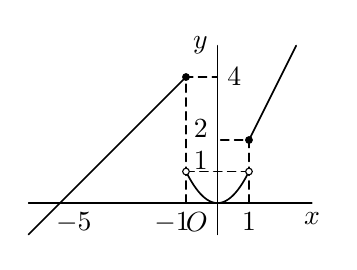
\begin{tikzpicture}[line cap=round,line join=round,scale=0.4]
      \draw[\myaxisarrow] (-6,0) -- (3,0) node[below] {$x$};
      \draw[\myaxisarrow] (0,-1) -- (0,5) node[left] {$y$};
      \draw[line width=0.6pt,smooth,samples=100] 
        plot[domain=-6:-1](\x,{\x+5})
        plot[domain=-1:1](\x,{(\x)^2})
        plot[domain=1:2.5](\x,{2*\x});
      \draw[line width=0.5pt, densely dashed] (-1,0)--(-1,4)--(0,4)
        (1,0)--(1,2)--(0,2) (-1,1)--(1,1);
      \draw[fill=white] (-1,1) circle(3pt) (1,1) circle(3pt);
      \draw[fill=black] (-1,4) circle(3pt) (1,2) circle(3pt);
      \draw (0,0) node[anchor=north east] {$O$} 
        (-5,0) node[below,xshift=5pt] {$-5$}
        (-1,0) node[below,xshift=-5pt] {$-1$} (1,0) node[below] {$1$}
        (0,1) node[left,yshift=4pt] {$1$} (0,2) node[left,yshift=4pt] {$2$}
        (0,4) node[right] {$4$};
    \end{tikzpicture}}
    
    (3) 分 $a\leqslant 1$, $-1<a<1$, $a\geqslant 1$ 解得, $a=-\frac92$ 或 $\pm\frac{\sqrt2}2$.
  \endsolution
  
  \begin{exercise}
    已知函数 $f(x)=|x-1|+2|x+1|$, 求其值域.
  \end{exercise}

  \beginsolution
    零点分段法讨论知
    \[f(x)=\begin{cases}
      1-3x, & x<-1,\\
      3-x, & -1\leqslant x\leqslant 1,\\
      3x-1, & x>1.\end{cases}\]
    分别求各段取值范围 (或作图), 可得值域 $[2,+\infty)$.
  \endsolution
  
  \begin{exercise}
    如图~\ref{fig-190414-2120}, 
    函数 $f(x)$ 的图象由两条射线和三条线段组成. 
    若对任意的 $x\in \mathbb{R}$, 都有 $f(x)>f(x-1)$, 
    则正实数 $a$ 的取值范围是\,?
    \begin{figure}[htb]
    \small
    \centering
    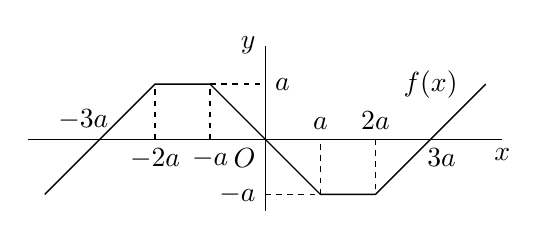
\begin{tikzpicture}[scale=0.7]
      \draw[\myaxisarrow] (-4.3,0) -- (4.3,0) node[below] {$x$};
      \draw[\myaxisarrow] (0,-1.3) -- (0,1.7) node[left] {$y$};
      \draw[line width=0.5pt] (-4,-1)--(-2,1)--(-1,1)--(1,-1)--(2,-1)--(4,1);
      \draw[line width=0.5pt,dash pattern= on 2pt off 2pt] 
        (-2,0)--(-2,1) (-1,0)--(-1,1)--(0,1) 
        (0,-1)--(1,-1)--(1,0) (2,0)--(2,-1);
      \draw (-3.3,0) node[above] {$-3a$} (-2,0) node[below] {$-2a$}
        (-1,0) node[below] {$-a$} (1,0) node[above] {$a$}
        (2,0) node[above] {$2a$} (3.2,0) node[below] {$3a$}
        (0,1) node[right] {$a$} (0,-1) node[left] {$-a$}
        (0,0) node[anchor=north east] {$O$}
        (3,1) node {$f(x)$};
    \end{tikzpicture}
    \caption{}\label{fig-190414-2120}
    \end{figure}
  \end{exercise}
  
  \beginsolution
    由 $f(x)$ 在 $[-2a,4a]$ 上的图象知, $0<6a<1$, 故 $a\in\Big(0,\frac16\Big)$.
  \endsolution
%%%%%%%%%%%%%%%%%%%%%%%%%%%%%